\documentclass[11pt,]{article}
\usepackage[left=1in,top=1in,right=1in,bottom=1in]{geometry}
\newcommand*{\authorfont}{\fontfamily{phv}\selectfont}
\usepackage[]{mathpazo}


  \usepackage[T1]{fontenc}
  \usepackage[utf8]{inputenc}



\usepackage{abstract}
\renewcommand{\abstractname}{}    % clear the title
\renewcommand{\absnamepos}{empty} % originally center

\renewenvironment{abstract}
 {{%
    \setlength{\leftmargin}{0mm}
    \setlength{\rightmargin}{\leftmargin}%
  }%
  \relax}
 {\endlist}

\makeatletter
\def\@maketitle{%
  \newpage
%  \null
%  \vskip 2em%
%  \begin{center}%
  \let \footnote \thanks
    {\fontsize{18}{20}\selectfont\raggedright  \setlength{\parindent}{0pt} \@title \par}%
}
%\fi
\makeatother




\setcounter{secnumdepth}{3}

\usepackage{longtable,booktabs}

\usepackage{graphicx,grffile}
\makeatletter
\def\maxwidth{\ifdim\Gin@nat@width>\linewidth\linewidth\else\Gin@nat@width\fi}
\def\maxheight{\ifdim\Gin@nat@height>\textheight\textheight\else\Gin@nat@height\fi}
\makeatother
% Scale images if necessary, so that they will not overflow the page
% margins by default, and it is still possible to overwrite the defaults
% using explicit options in \includegraphics[width, height, ...]{}
\setkeys{Gin}{width=\maxwidth,height=\maxheight,keepaspectratio}

\title{Patrones de Ecología Numérica Descritos por la Familia de Plantas
Fabaceae Mimosoideae en una Isla Subtropical, Cuenca del Mar Caribe.\\
\emph{Patterns of Numerical Ecology Described by Plants Family Fabaceae
Mimosoideae on a Subtropical Island, Caribbean Sea Basin}.\\  }



\author{\Large Welifer Junior Lebron Vicente\vspace{0.05in} \newline\normalsize\emph{Estudiante de Ciencias Geográficas, Universidad Autónoma de Santo
Domingo (UASD)}  }


\date{}

\usepackage{titlesec}

\titleformat*{\section}{\normalsize\bfseries}
\titleformat*{\subsection}{\normalsize\itshape}
\titleformat*{\subsubsection}{\normalsize\itshape}
\titleformat*{\paragraph}{\normalsize\itshape}
\titleformat*{\subparagraph}{\normalsize\itshape}

\titlespacing{\section}
{0pt}{36pt}{0pt}
\titlespacing{\subsection}
{0pt}{36pt}{0pt}
\titlespacing{\subsubsection}
{0pt}{36pt}{0pt}





\newtheorem{hypothesis}{Hypothesis}
\usepackage{setspace}

\makeatletter
\@ifpackageloaded{hyperref}{}{%
\ifxetex
  \PassOptionsToPackage{hyphens}{url}\usepackage[setpagesize=false, % page size defined by xetex
              unicode=false, % unicode breaks when used with xetex
              xetex]{hyperref}
\else
  \PassOptionsToPackage{hyphens}{url}\usepackage[unicode=true]{hyperref}
\fi
}

\@ifpackageloaded{color}{
    \PassOptionsToPackage{usenames,dvipsnames}{color}
}{%
    \usepackage[usenames,dvipsnames]{color}
}
\makeatother
\hypersetup{breaklinks=true,
            bookmarks=true,
            pdfauthor={Welifer Junior Lebron Vicente (Estudiante de Ciencias Geográficas, Universidad Autónoma de Santo
Domingo (UASD))},
             pdfkeywords = {Ecología Numérica, BCI, Análisis Forestal, Lenguaje R},  
            pdftitle={Patrones de Ecología Numérica Descritos por la Familia de Plantas
Fabaceae Mimosoideae en una Isla Subtropical, Cuenca del Mar Caribe.\\
\emph{Patterns of Numerical Ecology Described by Plants Family Fabaceae
Mimosoideae on a Subtropical Island, Caribbean Sea Basin}.\\},
            colorlinks=true,
            citecolor=blue,
            urlcolor=blue,
            linkcolor=magenta,
            pdfborder={0 0 0}}
\urlstyle{same}  % don't use monospace font for urls

% set default figure placement to htbp
\makeatletter
\def\fps@figure{htbp}
\makeatother

\usepackage{pdflscape} \newcommand{\blandscape}{\begin{landscape}}
\newcommand{\elandscape}{\end{landscape}}


% add tightlist ----------
\providecommand{\tightlist}{%
\setlength{\itemsep}{0pt}\setlength{\parskip}{0pt}}

\begin{document}
	
% \pagenumbering{arabic}% resets `page` counter to 1 
%
% \maketitle

{% \usefont{T1}{pnc}{m}{n}
\setlength{\parindent}{0pt}
\thispagestyle{plain}
{\fontsize{18}{20}\selectfont\raggedright 
\maketitle  % title \par  

}

{
   \vskip 13.5pt\relax \normalsize\fontsize{11}{12} 
\textbf{\authorfont Welifer Junior Lebron Vicente} \hskip 15pt \emph{\small Estudiante de Ciencias Geográficas, Universidad Autónoma de Santo
Domingo (UASD)}   

}

}








\begin{abstract}

    \hbox{\vrule height .2pt width 39.14pc}

    \vskip 8.5pt % \small 

\noindent Mi resumen


\vskip 8.5pt \noindent \emph{Keywords}: Ecología Numérica, BCI, Análisis Forestal, Lenguaje R \par

    \hbox{\vrule height .2pt width 39.14pc}



\end{abstract}


\vskip 6.5pt


\noindent  \section{Introducción}\label{introducciuxf3n}

El análisis de biodiversidad forestal viabiliza la obtención de
información sobre el comportamiento de las especies en su hábitat, los
efectos de cambios geoestacionarios, y las probables consecuencias de
actividades antrópicas en el ciclo vital de los bosques; cuya función en
el caso de los tropicales puede ser productiva (madera, fibra, leña,
productos no maderables); ambientales (regulación del clima, reserva de
biodiversidad, conservación de suelos y agua, etc.); y social
(subsistencia de poblamientos humanos locales y su cultura) (Montagnini,
Jordan, \& others, 2005).

La isla Barro Colorado (BCI), de coordenadas {[}9º 9' 0'`N, 79º 51' 0''
W{]}, es una plataforma basáltica miocénica sobre la que descansa un
bosque tropical primario compuesto por 305 especies arbóreas (Condit et
al., 1999). Esta fue el emplazamiento de ocho censos forestales
realizados por el Smithsonian Tropical Research Institute entre 1981 y
2015, donde la subfamilia \emph{Fabaceae Mimosoideae} representó el
5.9\% de las especies registradas en la parcela de 50 hectáreas
delimitada en 1980 {[}Cita3,WebP{]}.

\begin{figure}
\centering
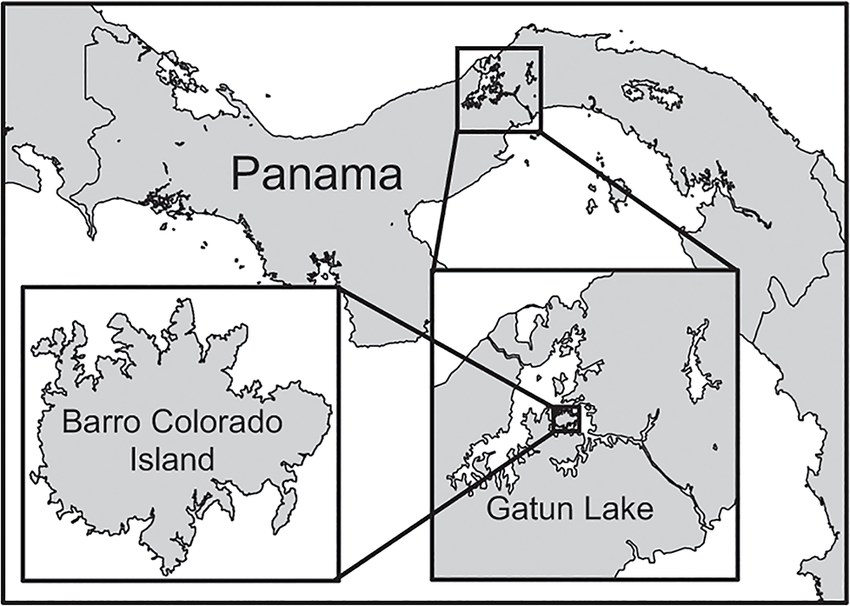
\includegraphics[width=0.50000\textwidth]{Map-of-Barro-Colorado-Island-BCI-Panama.png}
\caption{Isla Barro Colorado, Panamá (Baldeck et al., 2014).}
\end{figure}

El registro forestal de BCI forma parte de una serie de parcelas
permanentes delimitadas en distintas latitudes y longitudes, pero dentro
de la zona tropical. Estas parcelas poseen diferencias climáticas
específicas con el objetivo de contabilizar, supervisar y medir
variables demográficas que viabilicen realizar comparaciones atendiendo
a cuestionamientos científicos, registro detallado del comportamiento en
ecología vegetal o problemáticas resultantes de la intervención humana
en el equilibrio natural (Condit, 1998).

\begin{figure}
\centering
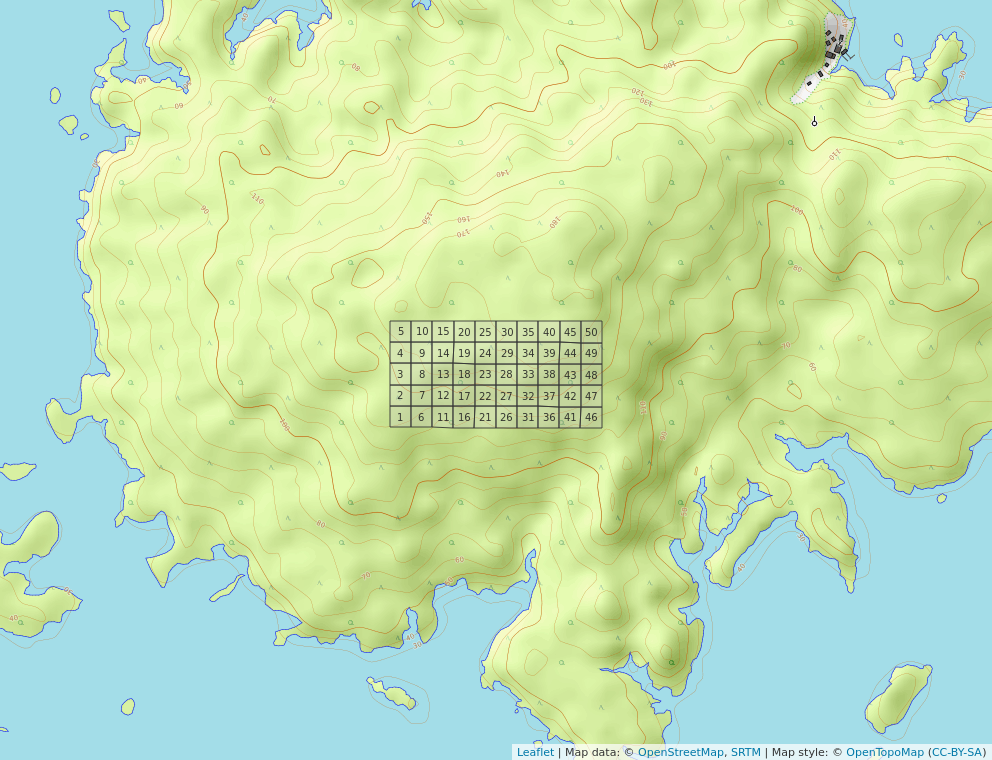
\includegraphics[width=0.50000\textwidth]{mapa_cuadros.png}
\caption{Área del censo forestal, Barro Colorado Island (1981-2015).}
\end{figure}

Las fabaceas concentran su diversidad en la franja tropical y
subtropical, aunque se encuentran ampliamente distribuidas por la
práctica totalidad de climas terrestres. Están presentes en zonas
árticas, litoral costero, ambientes alpinos, bosque lluvioso, bosque
estacional, sabanas, bosque seco, desiertos áridos, pantanos y
manglares. Poseen características especializadas que las hacen vitales
para el equilibrio ecológico y para la supervivencia del ser humano. El
88\% de las especies de esta familia pueden formar nódulos con bacterias
fijadoras de nitrógeno (rhizobia) para fijar el N2 en la atmósfera
mediante asociación simbiótica, fisiología rica en proteínas, etc.
Asimismo, sus semillas son empleadas para tratar células cancerígenas,
sus componentes químicos las hacen esenciales para diversos tipos de
industrias, y el grano de las leguminosas representa el 33\% del
nitrógeno necesario en la dieta de los seres humanos (Saikia, Nag,
Anurag, Chatterjee, \& Khan, 2020).

La subfamilia \emph{Mimosoideae} dentro del clado mimosoide es sumamente
variable, estando compuesta principalmente por árboles y arbustos de
flores asimétricas cigomorfas.

\begin{figure}
\centering
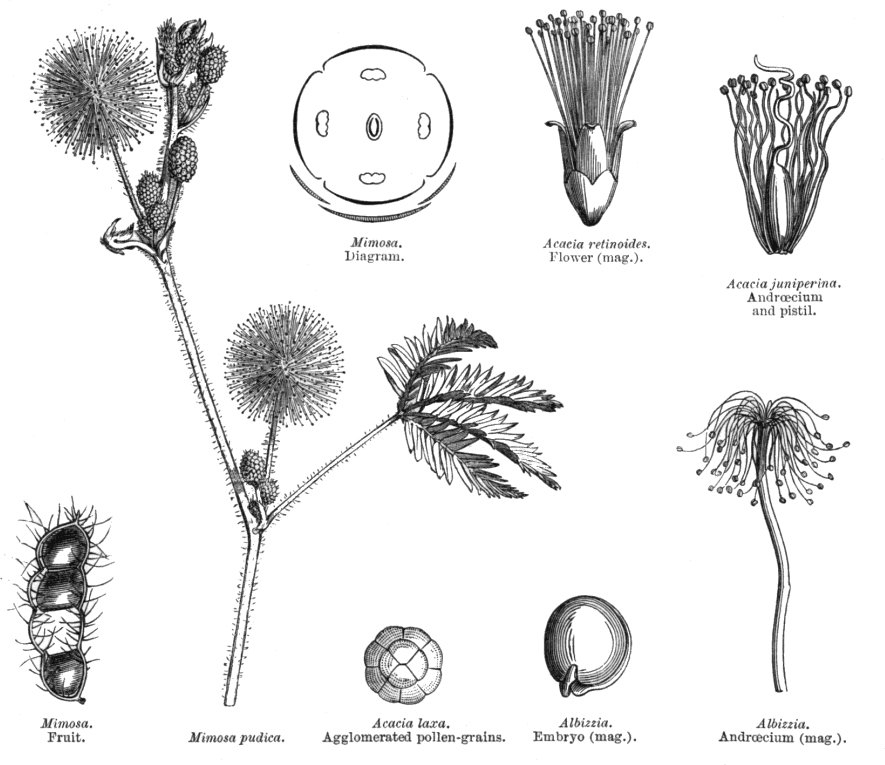
\includegraphics[width=0.50000\textwidth]{Grabado-Mimosoideae.png}
\caption{Grabado de fabaceas (Universiad de Toronto).}
\end{figure}

El clado filogenético mimosoide es propio de climas tropicales y
subtropicales, sus flores son simétricas con pétalos valvados y sus
especímenes tienen un gran número de estambres prominentes
(Hasanuzzaman, Araújo, \& Gill, 2020). En BCI se encuentran 18 de estas
especies.

Atendiendo a la flexibilidad en la distribución de las fabáceas, su
importancia económica, y social; se busca entender qué factores
ambientales intervienen en la proliferación, agrupamiento o decaimiento
de sus poblaciones en bosques tropicales que comparten características
con los hallados en República Dominicana, en esta ocasión tomando la
data cincuentenaria recolectada y provista por The Center for Tropical
Forest Science en BCI.

La ecología numérica es el campo de estudio que brinda las técnicas,
índices, y herramientas necesarias para obtener conclusiones a partir de
data forestal, animal, y biotopo. En ese sentido, R es un software de
código abierto y ambiente de programación que brinda una amplia variedad
de facilidades para el manejo, creación, y visualización gráfica de
ciencia de datos (Venables, Smith, Team, \& others, 2009).

\ldots

\section{Metodología}\label{metodologuxeda}

Una vez obtenida la data censal de Barro Colorado, se empleó el software
de código abierto R para realizar análisis estadísticos, gráficos,
matrices, y mapas.

Utilizando los paquetes \emph{vegan}, \emph{tydiverse}, y \emph{sf} se
extrajo la familia \emph{Fabaceae Mimosoideae} de la data censal, se
obtuvieron las estadísticas, gráficos lineales y diagramas de cajas. A
través de \emph{mapview} se crearon, proyectaron y almacenaron los
mapas. \emph{RColorBrewer} se empleó para obtener una gama de colores
más amplia en los gráficos y mapas (Batlle, 2020).

La caracterización geomorfológica se elaboró a partir del algoritmo
r.geomorphons por Batlle (2020) siguiendo el modelo de Jasiewicz \&
Stepinski (2013). (Ver figuras \ref{Geomorf3} y \ref{Geomorf2})

\begin{figure}
\centering
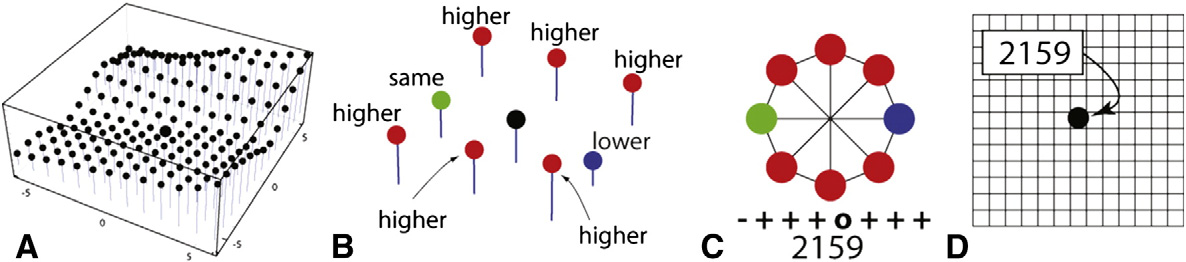
\includegraphics[width=1.00000\textwidth]{Geomorf3.png}
\caption{Modelo desarrollado por Jasiewicz \& Stepinski (2013) para la
caracterización del relieve.\label{Geomorf3}}
\end{figure}

\begin{figure}
\centering
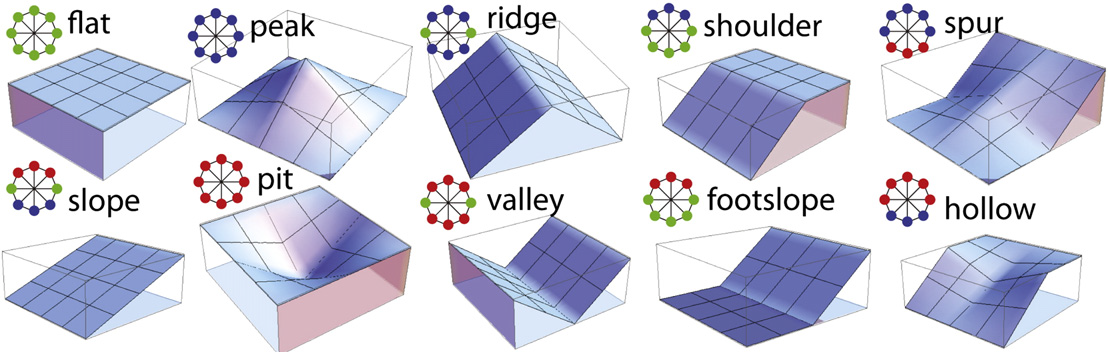
\includegraphics[width=1.00000\textwidth]{Geomor2.png}
\caption{Ejemplos de las variantes de relive más comunes obtenidas a
través del algoritmo (ibidem).\label{Geomorf2}}
\end{figure}

Diversos estudios fueron tomados en cuenta para la clasificación de
hábitats, se empleó la categorización realizada por Harms, Condit,
Hubbell, \& Foster (2001) partiendo del resumen y análisis de la data
compilada en 16,6 años. (Ver tabla \ref{tab:hábitat})

\begin{longtable}[]{@{}lcc@{}}
\caption{Clasificación de hábitats, parcela permanente BCI (Harms et
al., 2001).\label{tab:hábitat}}\tabularnewline
\toprule
Hábitat & Pendiente (grados) & Elevación (metros)\tabularnewline
\midrule
\endfirsthead
\toprule
Hábitat & Pendiente (grados) & Elevación (metros)\tabularnewline
\midrule
\endhead
Bosque adulto - Meseta baja & \textless{}7 &
\textless{}152\tabularnewline
Bosque adulto - Meseta alta & \textless{}7 & = o
\textgreater{}152\tabularnewline
Bosque adulto - Pendiente & = o \textgreater{}7 & Todas\tabularnewline
Bosque adulto - Área pantanosa & Todas & Todas\tabularnewline
Bosque adulto - Ribera fluvial & Todas & Todas\tabularnewline
Bosque joven & Todas & Todas\tabularnewline
Hábitats mixtos & Todas & Todas\tabularnewline
\bottomrule
\end{longtable}

Mapas de ubicación, abundancia de individuos, riqueza de especies,
agrupamiento de parcelas, pH, nitrógeno y otras variables presentes en
el relieve, clima, y edafología del lugar se emplearon para determinar
patrones asociativos entre las especies de fabáceas.

Se determinó la asociación interespecífica y de sitios muestrales
mediante los métodos R y Q respectivamente. En el modo Q se obtuvo
mediante la métrica de distancia euclidea o similaridad de Jaccard,
verificando la paradoja de orlóci (1978); transformación de cuerdas
(\emph{chord}); \emph{ji}-cuadrado; y \emph{Hellinger}. Mientras que en
el modo R se calculó el índice de correlación de Pearson aplicando la
transformación de \emph{chi} para corregir alteraciones producidas por
outliers en los datos; la matriz de comunidad transpuesta convertida a
binaria (presencia/ausencia) para calcular distancia entre especies con
la similaridad de Jaccard; el índice \emph{rho} de Sperman y \emph{tau}
de Kendall (Batlle, 2020).

\ldots

\section{Resultados}\label{resultados}

La parcela de 50ha en BCI posee 3847 individuos de la familia
\emph{Fabaceae Mimosoideae} agrupados en 18 especies distribuidas de
forma aleatoria en 50 sitios de 1ha cada uno. La especie más abundante
es \emph{Inga Marginata} {[}767{]}, seguida de cerca por \emph{Inga
Umbellifera} {[}765{]}; mientras que la más escasa es \emph{Cojoba
Rufescens} {[}2{]}, seguida de \emph{Inga Oerstediana} {[}4{]}. La
abundancia especifica acorde a una organización ascendente por número de
individuos presenta una mediana de 57 individuos {[}\emph{Inga Punctata}
e \emph{Inga Laurina}{]}, siendo la mitad más pobre de especies el
equivalente a un 5.82\% {[}224{]} y la mitad más presente el 94.18\%
{[}3623{]}. La riqueza de especies por cuadrante evidencia una
distribución también desproporcional, el C26 presenta la riqueza más
débil {[}5{]} y el C30 la más fuerte {[}13{]}. No obstante, aunque no
existe relación directa entre la riqueza y la abundancia por cuadrante,
en C26 coíncide y en algunos otros cuadros puede existir cierta
aproximación.

(ver tabla \ref{tab:abun_sp} y figura \ref{fig:abun_sp_q})

\begin{longtable}[]{@{}lr@{}}
\caption{\label{tab:abun_sp}Abundancia por especie de la familia
\emph{Fabaceae-Mimosoideae}.}\tabularnewline
\toprule
Latin & n\tabularnewline
\midrule
\endfirsthead
\toprule
Latin & n\tabularnewline
\midrule
\endhead
Inga marginata & 767\tabularnewline
Inga umbellifera & 765\tabularnewline
Inga acuminata & 606\tabularnewline
Inga nobilis & 557\tabularnewline
Inga goldmanii & 297\tabularnewline
Inga thibaudiana & 232\tabularnewline
Inga sapindoides & 197\tabularnewline
Inga pezizifera & 145\tabularnewline
Inga laurina & 57\tabularnewline
Inga punctata & 57\tabularnewline
Inga cocleensis & 54\tabularnewline
Acacia melanoceras & 48\tabularnewline
Inga spectabilis & 20\tabularnewline
Abarema macradenia & 19\tabularnewline
Enterolobium schomburgkii & 12\tabularnewline
Inga ruiziana & 8\tabularnewline
Inga oerstediana & 4\tabularnewline
Cojoba rufescens & 2\tabularnewline
\bottomrule
\end{longtable}

\begin{figure}
\centering
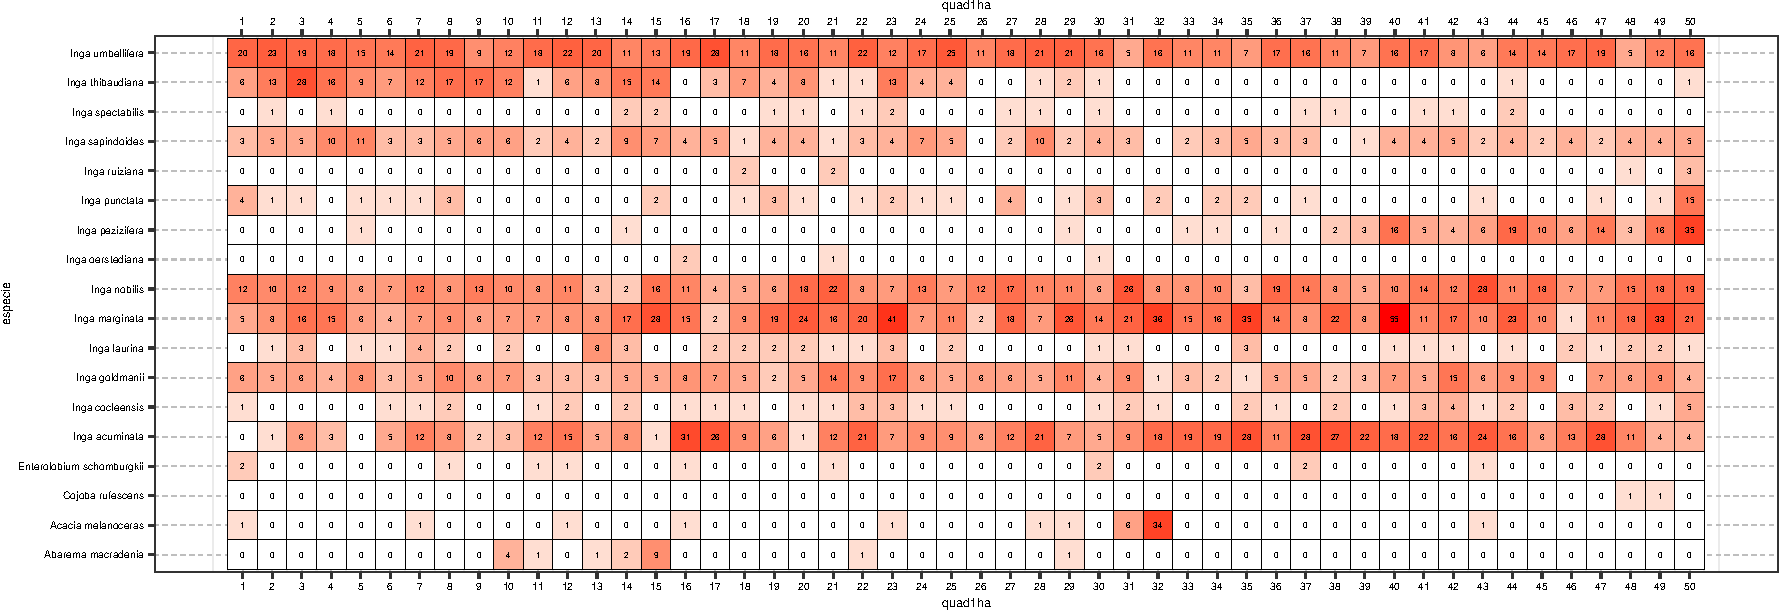
\includegraphics{manuscrito_files/figure-latex/unnamed-chunk-3-1.pdf}
\caption{\label{fig:abun_sp_q}Abundancia por especie por quadrat}
\end{figure}

El terreno eminentemente describe una geomorfología en vertiente, siendo
esta característica la más destacada en el 88\% de los C 1Ha; en tanto
que el 12\% restante describe una geomorfología donde predomina el
relieve llano. La parcela madre está compuesta en un 52\% por bosque
adulto en meseta baja distribuido ampliamente, un 24\% por bosque adulto
en pendiente con presencia marcada en las parcelas {[}C41-C45{]}, un
16\% por bosque adulto en meseta alta concentrado en las parcelas
{[}C3-C34; C37-C40{]}, mientras que el 8\% restante hábitat pantanoso y
bosque jovén en forma equitativa. No parece existir una relación directa
entre la morfología del espacio y un determinado hábitat, exeptuando el
bosque joven que se encuentra tanto en llanura como en vertiente de
forma considerable. En general, se percibe un leve aumento de la riqueza
específica a medida que aumenta la abundancia de individuos; destacando
la abundante riqueza de especies en el hábitat pantanoso, su pobreza en
el bosque adulto en zona alta, la abundancia marcada el bosque adulto en
zona baja y su riqueza equilibrada . (Ver Gráficos lineales 1 y 2).

Insertar Gráfs\_Regresión\_Lineal\_aed\_2.

----Podría interpretar mejor el boxplot---- *Sería interesante dedicar
un acápite para la descripción de la composición mineral del suelo,
hacer un ançalisis de las variables de elementos tomando en cuenta 5 C
con más y 5 C con menos presencia.

Las fabáceas

\section{Discusión}\label{discusiuxf3n}

\section{Agradecimientos}\label{agradecimientos}

\section{Información de soporte}\label{informaciuxf3n-de-soporte}

\ldots

\section{\texorpdfstring{\emph{Script}
reproducible}{Script reproducible}}\label{script-reproducible}

\ldots

\section*{Referencias}\label{referencias}
\addcontentsline{toc}{section}{Referencias}

\hypertarget{refs}{}
\hypertarget{ref-inproceedings}{}
Baldeck, C., Asner, G., Martin, R., Anderson, C., Knapp, D., Kellner,
J., \& Wright, S. J. (2014). Operational tree species mapping in a
diverse tropical forest with airborne imaging spectroscopy. \emph{PloS
one}, \emph{10}. \url{https://doi.org/10.1371/journal.pone.0118403}

\hypertarget{ref-jose_ramon_martinez_batlle_2020_4402362}{}
Batlle, J. R. M. (2020). biogeografia-master/scripts-de-analisis-BCI:
Long coding sessions (Version v0.0.0.9000).
\url{https://doi.org/10.5281/zenodo.4402362}

\hypertarget{ref-condit1998tropical}{}
Condit, R. (1998). \emph{Tropical forest census plots: Methods and
results from barro colorado island, panama and a comparison with other
plots}. Springer Science \& Business Media.

\hypertarget{ref-condit1999dynamics}{}
Condit, R., Ashton, P. S., Manokaran, N., LaFrankie, J. V., Hubbell, S.
P., \& Foster, R. B. (1999). Dynamics of the forest communities at pasoh
and barro colorado: Comparing two 50--ha plots. \emph{Philosophical
Transactions of the Royal Society of London. Series B: Biological
Sciences}, \emph{354}(1391), 1739--1748.

\hypertarget{ref-harms2001habitat}{}
Harms, K. E., Condit, R., Hubbell, S. P., \& Foster, R. B. (2001).
Habitat associations of trees and shrubs in a 50-ha neotropical forest
plot. \emph{Journal of Ecology}, \emph{89}(6), 947--959.

\hypertarget{ref-hasanuzzaman2020plant}{}
Hasanuzzaman, M., Araújo, S., \& Gill, S. S. (2020). \emph{The plant
family fabaceae: Biology and physiological responses to environmental
stresses}. Springer Nature.

\hypertarget{ref-jasiewicz2013geomorphons}{}
Jasiewicz, J., \& Stepinski, T. F. (2013). Geomorphons---a pattern
recognition approach to classification and mapping of landforms.
\emph{Geomorphology}, \emph{182}, 147--156.

\hypertarget{ref-montagnini2005tropical}{}
Montagnini, F., Jordan, C. F., \& others. (2005). \emph{Tropical forest
ecology: The basis for conservation and management}. Springer Science \&
Business Media.

\hypertarget{ref-saikia2020tropical}{}
Saikia, P., Nag, A., Anurag, S., Chatterjee, S., \& Khan, M. L. (2020).
Tropical legumes: Status, distribution, biology and importance. In
\emph{The plant family fabaceae} (pp. 27--41). Springer.

\hypertarget{ref-venables2009introduction}{}
Venables, W. N., Smith, D. M., Team, R. D. C., \& others. (2009).
\emph{An introduction to r}. Citeseer.




\newpage
\singlespacing 
\end{document}
